\usetikzlibrary{calc}

\definecolor{DarkPink}{rgb}{0.55, 0.05, 0.37}

\newcommand*{\GridSize}{8}

\newcommand*{\ColorCells}[1]{% #1 = list of x/y/color
  \foreach \x/\y/\color/\text in {#1} {
    \node [fill=\color, draw=black, thick ,minimum size=1cm, line width=.8pt] 
      at (\x-.5,\GridSize+0.5-\y) [text=black] {\text};
    }%
}%

\tikzset{near start abs/.style={xshift=1cm}}
%%%%%


%\listfiles
\scalebox{0.42}{ %%% scale it
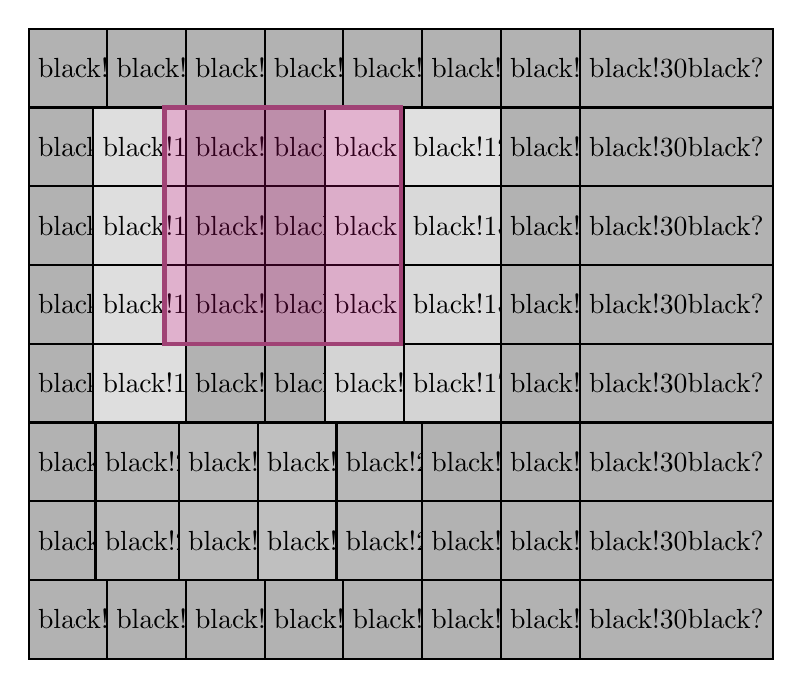
\begin{tikzpicture}
    \begin{scope}[thick,local bounding box=name]
    
         \ColorCells{
            1/1/black!30/?,
            1/2/black!30/?,
            1/3/black!30/?,
            1/4/black!30/?,
            1/5/black!30/?,
            1/6/black!30/?,
            1/7/black!30/?,
            1/8/black!30/?,
            2/1/black!30/0,
            2/2/black!13/140,
            2/3/black!13/140,
            2/4/black!13/140,
            2/5/black!13/140,
            2/6/black!28/-10,
            2/7/black!28/-10,
            2/8/black!30/0,
            3/1/black!30/0,
            3/2/black!30/0,
            3/3/black!30/0,
            3/4/black!30/0,
            3/5/black!30/0,
            3/6/black!27/20,
            3/7/black!27/20,
            3/8/black!30/0,
            4/1/black!30/0,
            4/2/black!30/0,
            4/3/black!30/0,
            4/4/black!30/0,
            4/5/black!30/0,
            4/6/black!25/40,
            4/7/black!25/40,
            4/8/black!30/0,
            5/1/black!30/0,
            5/2/black!12/-150,
            5/3/black!15/-120,
            5/4/black!15/-120,
            5/5/black!17/-110,
            5/6/black!28/10,
            5/7/black!28/10,
            5/8/black!30/0,
            6/1/black!30/0,
            6/2/black!12/-150,
            6/3/black!15/-120,
            6/4/black!15/-120,
            6/5/black!17/-110,
            6/6/black!30/0,
            6/7/black!30/0,
            6/8/black!30/0,
            7/1/black!30/0,
            7/2/black!30/0,
            7/3/black!30/0,
            7/4/black!30/0,
            7/5/black!30/0,
            7/6/black!30/0,
            7/7/black!30/0,
            7/8/black!30/0,
            8/1/black!30/?,
            8/2/black!30/?,
            8/3/black!30/?,
            8/4/black!30/?,
            8/5/black!30/?,
            8/6/black!30/?,
            8/7/black!30/?,
            8/8/black!30/?
         }
   \draw [draw=magenta!60!black,fill=magenta, fill opacity=0.2,ultra thick](1,7) rectangle (4,4);
    \end{scope}
\end{tikzpicture}
} %%% case